\documentclass[10pt, aspectratio=169]{beamer}
\usefonttheme{professionalfonts}

\mode<presentation>
{
  \usetheme{Berkeley}
  \usecolortheme{beaver}
  \usefonttheme{default}
  \setbeamertemplate{navigation symbols}{}
  \setbeamertemplate{caption}[numbered]
} 

\setbeamertemplate{footline}{%
  \leavevmode%
  \hbox{%
    \begin{beamercolorbox}[wd=.85\paperwidth,ht=2.5ex,dp=1ex,left]{author in head/foot}%
      \usebeamerfont{author in head/foot}Maxx Seminario, Electronic Circuits, Spring 2026%
    \end{beamercolorbox}%
    \begin{beamercolorbox}[wd=.15\paperwidth,ht=2.5ex,dp=1ex,right]{date in head/foot}%
      \hspace*{0.5em}\insertframenumber{} / \inserttotalframenumber\hspace*{0.5em}%
    \end{beamercolorbox}%
  }%
  \vskip0pt%
}

\usepackage[english]{babel}
\usepackage[utf8x]{inputenc}
\usepackage{tikz}
\usetikzlibrary{shapes.geometric}
\usepackage{pgfplots}
\usepackage{array}
\usepackage{makecell}
\usepackage{verbatim}
\usepackage{graphicx}
\usepackage{subcaption}
\usepackage{amsfonts}
\usepackage{amsmath}
\usepackage{bm}
\usepackage{epstopdf}
\usepackage{circuitikz}
\usepackage{caption}
\usepackage{multirow}
\captionsetup{compatibility=false}
\usepackage[absolute,overlay]{textpos}
\usetikzlibrary{calc}
\usetikzlibrary{pgfplots.fillbetween, backgrounds}
\usetikzlibrary{positioning}
\usetikzlibrary{pgfplots.groupplots}
\usetikzlibrary{plotmarks}
\usetikzlibrary{calc}
\usetikzlibrary{patterns}
\usepgfplotslibrary{groupplots}
\pgfplotsset{compat=newest} 

\usepackage{hyperref}
\definecolor{BeaverRed}{RGB}{179,38,38} 
\hypersetup{
    colorlinks=true,
    linkcolor=BeaverRed,
    filecolor=magenta,      
    urlcolor=cyan,
}

% Added by Maxx Seminario - for colored icons in itemize labels
\usepackage{wasysym} 
\newcommand{\neutralface}{%
  \tikz[baseline=-0.6ex]{
    \draw (0,0) circle (0.9ex);
    \fill (-0.35ex,0.25ex) circle (0.12ex);
    \fill ( 0.35ex,0.25ex) circle (0.12ex);
    \draw (-0.35ex,-0.25ex) -- (0.35ex,-0.25ex);
  }%
}

\newcommand{\baditem}{\textcolor{red! 70! black}{\frownie}}
\newcommand{\gooditem}{\textcolor{green!60!black}{\smiley}}
\newcommand{\mehitem}{\textcolor{orange!80!black}{\neutralface}}

% =========================
% Solution toggle 
% =========================
\newif\ifshowsolutions
\showsolutionstrue   %  compile WITH solutions
%\showsolutionsfalse %  compile WITHOUT solutions

% =========================
% Document Information
% =========================
\title[MOSFET Structure]{MOSFET Device Structure and Physical Operation}
\subtitle{Unit 5: Field-Effect Transistors}
\author{Maxx Seminario}
\institute{University of Nebraska-Lincoln}
\date{Spring 2026}

\begin{document}

\begin{frame}
  \titlepage
\end{frame}

\section{Introduction}

\begin{frame}{Lecture Overview}
    
    \begin{columns}[t]
    \column{0.48\textwidth}
        \textbf{What is a MOSFET?}
        
        \begin{itemize}
            \item \textbf{M}etal-\textbf{O}xide-\textbf{S}emiconductor \textbf{F}ield-\textbf{E}ffect \textbf{T}ransistor
            \item Three-terminal voltage-controlled device
            \item Current controlled by electric field
            \item Foundation of modern integrated circuits
        \end{itemize}
        
        \textbf{Why MOSFETs?}
        
        \begin{itemize}
            \item Low power consumption
            \item High input impedance
            \item Scalable to nanometer dimensions
            \item Digital logic (billions per chip)
            \item Analog circuits (amplifiers)
        \end{itemize}
        
    \column{0.48\textwidth}
        \begin{block}{Lecture Objectives}
            \begin{itemize}
                \item Understand MOSFET device structure
                \item Analyze physical operation principles
                \item Study operating regions (cutoff, linear, saturation)
                \item Derive I-V characteristics
                \item Understand field effect and channel modulation
            \end{itemize}
        \end{block}
        

    \end{columns}
    
\end{frame}

\section{MOSFET Structure}

\begin{frame}{MOSFET Device Structure: n-Channel (NMOS)}
    
    \begin{columns}[t]
    \column{0.38\textwidth}
        \textbf{Key Components}:
        \begin{itemize}
            \item \textbf{Gate}: Controls channel
            \item \textbf{Source/Drain}: n$^+$ regions in p-substrate
            \item \textbf{Oxide}: Insulator (SiO$_2$)
            \item \textbf{Channel}: Conducting path (induced)
        \end{itemize}
        
        % \vspace{0.5cm}
        
        \textbf{Parameters}:
        \begin{itemize}
            \item $L$: Channel length
            \item $W$: Channel width (into page)
            \item $t_{ox}$: Oxide thickness
            \item $C_{ox} = \epsilon_{ox}/t_{ox}$: Oxide capacitance
        \end{itemize}
        
    \column{0.58\textwidth}
        \begin{center}
        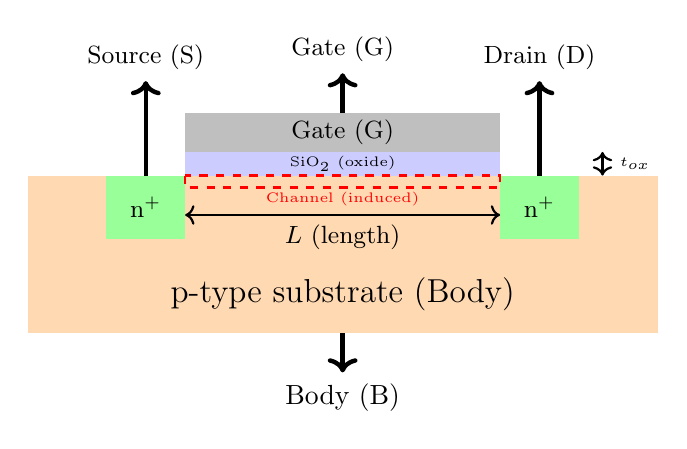
\begin{tikzpicture}[scale=1.0]
            % Substrate (p-type)
            \fill[orange!30] (0,-2) rectangle (8,0);
            \node[font=\large] at (4,-1.5) {p-type substrate (Body)};
            
            % Source n+ region 
            \fill[green!40] (1,-0.8) rectangle (2,0);
            \node[font=\small] at (1.5,-0.4) {n$^+$};
            
            % Drain n+ region 
            \fill[green!40] (6,-0.8) rectangle (7,0);
            \node[font=\small] at (6.5,-0.4) {n$^+$};
            
            % Gate oxide 
            \fill[blue!20] (2,0) rectangle (6,0.3);
            \node[font=\tiny] at (4,0.15) {SiO$_2$ (oxide)};
            
            % Gate metal 
            \fill[gray!50] (2,0.3) rectangle (6,0.8);
            \node[font=\small] at (4,0.55) {Gate (G)};
            
            % Channel region
            \draw[dashed, thick, red] (2,0) rectangle (6,-0.15);
            \node[font=\tiny, red] at (4,-0.3) {Channel (induced)};
            
            % Terminals
            \draw[->, ultra thick] (1.5,0) -- (1.5,1.2) node[above, font=\small] {Source (S)};
            \draw[->, ultra thick] (6.5,0) -- (6.5,1.2) node[above, font=\small] {Drain (D)};
            \draw[->, ultra thick] (4,0.8) -- (4,1.3) node[above, font=\small] {Gate (G)};
            \draw[->, ultra thick] (4,-2) -- (4,-2.5) node[below] {Body (B)};
            
            % Dimensions
            \draw[<->, thick] (2,-0.5) -- (6,-0.5);
            \node[below, font=\small] at (4,-0.5) {$L$ (length)};
            
            \draw[<->, thick] (7.3,0) -- (7.3,0.3);
            \node[right, font=\tiny] at (7.4,0.15) {$t_{ox}$};
            
        \end{tikzpicture}
        \end{center}
        
    \end{columns}
    
\end{frame}

\begin{frame}{n-Channel vs p-Channel MOSFET}
    
    \begin{columns}[t]
    \column{0.48\textwidth}
        \textbf{n-Channel (NMOS)}
        
        \begin{center}
        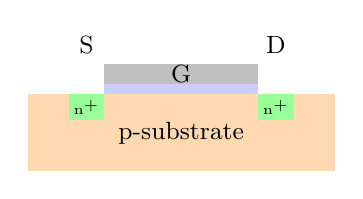
\begin{tikzpicture}[scale=0.65]
            % Substrate
            \fill[orange!30] (0,-1.5) rectangle (6,0);
            \node[font=\small] at (3,-0.75) {p-substrate};
            
            % Source/Drain (embedded in substrate, flush with surface)
            \fill[green!40] (0.8,-0.5) rectangle (1.5,0);
            \node[font=\tiny] at (1.15,-0.25) {n$^+$};
            \fill[green!40] (4.5,-0.5) rectangle (5.2,0);
            \node[font=\tiny] at (4.85,-0.25) {n$^+$};
            
            % Oxide (on top of substrate)
            \fill[blue!20] (1.5,0) rectangle (4.5,0.2);
            
            % Gate (on top of oxide)
            \fill[gray!50] (1.5,0.2) rectangle (4.5,0.6);
            \node[font=\small] at (3,0.4) {G};
            
            % Labels
            \node[above, font=\small] at (1.15,0.6) {S};
            \node[above, font=\small] at (4.85,0.6) {D};
            
        \end{tikzpicture}
        \end{center}
        
        \begin{itemize}
            \item p-type substrate
            \item n$^+$ source and drain
            \item Electrons are carriers
            \item Positive $V_{GS}$ creates channel
        \end{itemize}
        
    \column{0.48\textwidth}
        \textbf{p-Channel (PMOS)}
        
        \begin{center}
        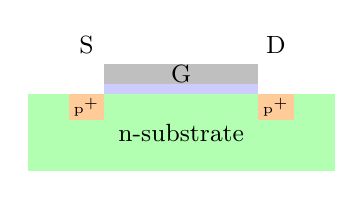
\begin{tikzpicture}[scale=0.65]
            % Substrate
            \fill[green!30] (0,-1.5) rectangle (6,0);
            \node[font=\small] at (3,-0.75) {n-substrate};
            
            % Source/Drain (embedded in substrate, flush with surface)
            \fill[orange!40] (0.8,-0.5) rectangle (1.5,0);
            \node[font=\tiny] at (1.15,-0.25) {p$^+$};
            \fill[orange!40] (4.5,-0.5) rectangle (5.2,0);
            \node[font=\tiny] at (4.85,-0.25) {p$^+$};
            
            % Oxide (on top of substrate)
            \fill[blue!20] (1.5,0) rectangle (4.5,0.2);
            
            % Gate (on top of oxide)
            \fill[gray!50] (1.5,0.2) rectangle (4.5,0.6);
            \node[font=\small] at (3,0.4) {G};
            
            % Labels
            \node[above, font=\small] at (1.15,0.6) {S};
            \node[above, font=\small] at (4.85,0.6) {D};
            
        \end{tikzpicture}
        \end{center}
        
        \begin{itemize}
            \item n-type substrate
            \item p$^+$ source and drain
            \item Holes are carriers
            \item Negative $V_{GS}$ creates channel
        \end{itemize}
        
    \end{columns}
    
    \vspace{0.3cm}
    
    \begin{block}{Focus of This Lecture}
        We will focus on \textbf{n-channel enhancement-mode MOSFETs}. Concepts apply to PMOS with appropriate sign changes.
    \end{block}
    
\end{frame}

\begin{frame}{MOSFET Symbol}
    
    \begin{columns}[t]
    \column{0.48\textwidth}
        \textbf{n-Channel MOSFET}
        
        \begin{center}
        \begin{circuitikz}[scale=1.5]
            % NMOS symbol with arrow into source
            \draw (0,0) node[nmos, arrowmos, thick] (nmos) {};
            
            % Labels
            \node[left] at (nmos.gate) {G};
            \node[above] at (nmos.drain) {D};
            \node[below] at (nmos.source) {S};
            
        \end{circuitikz}
        \end{center}
        
        \vspace{0.3cm}
        
        \textbf{Conventions}:
        \begin{itemize}
            \item Arrow points \textbf{out of} channel (n-type)
            \item Source: lower potential terminal
            \item Drain: higher potential terminal
        \end{itemize}
        
    \column{0.48\textwidth}
        \textbf{p-Channel MOSFET}
        
        \begin{center}
        \begin{circuitikz}[scale=1.5]
            % PMOS symbol with arrow out of source
            \draw (0,0) node[pmos, arrowmos, thick] (pmos) {};
            
            % Labels
            \node[left] at (pmos.gate) {G};
            \node[above, yshift=-0.5cm] at (pmos.drain) {D};
            \node[below, yshift=0.5cm] at (pmos.source) {S};
            
        \end{circuitikz}
        \end{center}
        
        \vspace{0.3cm}
        
        \textbf{Conventions}:
        \begin{itemize}
            \item Arrow points \textbf{into} channel (p-type)
            \item Source: higher potential terminal
            \item Drain: lower potential terminal
        \end{itemize}
        
    \end{columns}
    
\end{frame}

\section{Operating Principles}

\begin{frame}{Operating Principle: The Field Effect}
    
    \begin{columns}[t]
    \column{0.48\textwidth}
        \textbf{Key Concept}:
        \begin{itemize}
            \item Gate - oxide - substrate form capacitor
            \item Electric field attracts carriers to oxide interface
            \item Forms conducting \textbf{inversion layer}
            \item Channel connects source to drain
            \item Current flows when $V_{GS} > V_{th}$
        \end{itemize}
        
        % \vspace{0.3cm}
        
        \textbf{Threshold Voltage} ($V_{th}$):
        \begin{itemize}
            \item Minimum $V_{GS}$ to create channel
            \item Typically 0.3V to 1.0V for NMOS
        \end{itemize}
        
    \column{0.48\textwidth}
        \begin{center}
        \textbf{Channel Formation (NMOS)}
        
        \vspace{0.2cm}
        
        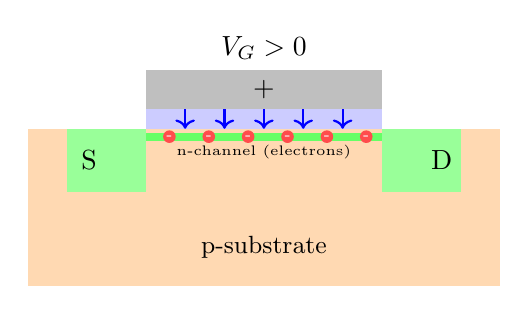
\begin{tikzpicture}[scale=1.0]
            % Substrate
            \fill[orange!30] (0,-2) rectangle (6,0);
            \node[font=\small] at (3,-1.5) {p-substrate};
            
            % Source/Drain 
            \fill[green!40] (0.5,-0.8) rectangle (1.5,0);
            \fill[green!40] (4.5,-0.8) rectangle (5.5,0);
            
            % Oxide 
            \fill[blue!20] (1.5,0) rectangle (4.5,0.25);
            
            % Gate 
            \fill[gray!50] (1.5,0.25) rectangle (4.5,0.75);
            \node at (3,0.5) {+};
            
            % Channel 
            \fill[green!60] (1.5,-0.05) rectangle (4.5,-0.15);
            \node[font=\tiny] at (3,-0.3) {n-channel (electrons)};
            
            % Electric field lines
            \foreach \x in {2, 2.5, 3, 3.5, 4} {
                \draw[->, thick, blue] (\x,0.25) -- (\x,0);
            }
            
            % Electrons in channel
            \foreach \x in {1.8, 2.3, 2.8, 3.3, 3.8, 4.3} {
                \fill[red!70] (\x,-0.1) circle (0.08cm);
                \node[white, font=\tiny] at (\x,-0.1) {-};
            }
            
            % Labels
            \node[above] at (3,0.75) {$V_G > 0$};
            \node[left] at (1,-0.4) {S};
            \node[right] at (5,-0.4) {D};
            
        \end{tikzpicture}
        \end{center}
        
    \end{columns}
    
    \vspace{0.2cm}
    
    \begin{block}{Field Effect}
        Positive gate voltage attracts electrons to the surface, forming a conducting channel of mobile carriers (electrons in inversion layer).
    \end{block}
    
\end{frame}

\section{Operating Regions}

\begin{frame}{MOSFET Operating Regions}

    \vspace{-0.5cm}
    
    \begin{center}
    \begin{tabular}{|l|c|c|p{5cm}|}
    \hline
    \textbf{Region} & \textbf{Condition} & \textbf{Current} & \textbf{Description} \\
    \hline
    \hline
    \textbf{Cutoff} & $V_{GS} < V_{th}$ & $I_{DS} = 0$ & No channel formed, transistor OFF \\
    \hline
    \textbf{Linear (Triode)} & \shortstack{$V_{GS} > V_{th}$ \\ and \\ $V_{DS} < V_{GS} - V_{th}$} & $I_{DS} \propto V_{DS}$ & Channel exists throughout, acts like resistor \\
    \hline
    \textbf{Saturation} & \shortstack{$V_{GS} > V_{th}$ \\ and \\ $V_{DS} \geq V_{GS} - V_{th}$} & $I_{DS}$ constant & Channel pinched off at drain, current saturates \\
    \hline
    \end{tabular}
    \end{center}
    
    \begin{columns}[t]
    \column{0.48\textwidth}
        \textbf{Key Voltages}:
        \begin{itemize}
            \item $V_{GS}$: Gate-to-Source voltage
            \item $V_{DS}$: Drain-to-Source voltage
            \item $V_{th}$: Threshold voltage
            \item $V_{OV} = V_{GS} - V_{th}$: Overdrive voltage
        \end{itemize}
        
    \column{0.48\textwidth}
        \textbf{Operating Region Selection}:
        \begin{itemize}
            \item \textbf{Digital}: Cutoff (Off), Saturation (On)
            \item \textbf{Analog amplifiers}: Saturation region
            \item \textbf{Switches}: Linear region (low $R_{DS,on}$)
        \end{itemize}
        
    \end{columns}
    
\end{frame}

\begin{frame}{Cutoff Region: $V_{GS} < V_{th}$}
    
    \begin{columns}[t]
    \column{0.48\textwidth}
        \textbf{Conditions}:
        \begin{itemize}
            \item $V_{GS} < V_{th}$
            \item Gate voltage too low to invert substrate surface
            \item No inversion layer or channel
        \end{itemize}
        
        \textbf{Characteristics}:
        \begin{itemize}
            \item $I_{DS} \approx 0$ 
            \item Transistor is off
            \item Source and drain electronically isolated
            \item Only leakage current flows (nA range)
        \end{itemize}
        
        \vspace{0.3cm}
        
        \textbf{Equation}:
        $$I_{DS} \approx 0 \quad \text{for } V_{GS} < V_{th}$$
        
    \column{0.48\textwidth}
        \begin{center}
        \textbf{Device Cross-Section}
        
        \vspace{0.2cm}
        
        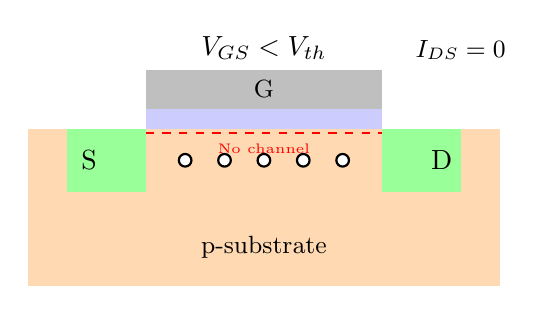
\begin{tikzpicture}[scale=1.0]
            % Substrate
            \fill[orange!30] (0,-2) rectangle (6,0);
            \node[font=\small] at (3,-1.5) {p-substrate};
            
            % Source/Drain 
            \fill[green!40] (0.5,-0.8) rectangle (1.5,0);
            \fill[green!40] (4.5,-0.8) rectangle (5.5,0);
            
            % Oxide 
            \fill[blue!20] (1.5,0) rectangle (4.5,0.25);
            
            % Gate 
            \fill[gray!50] (1.5,0.25) rectangle (4.5,0.75);
            \node[font=\small] at (3,0.5) {G};
            
            % NO channel 
            \draw[dashed, red, thick] (1.5,-0.05) -- (4.5,-0.05);
            \node[font=\tiny, red] at (3,-0.25) {No channel};
            
            % Holes in substrate
            \foreach \x in {2, 2.5, 3, 3.5, 4} {
                \draw[fill=white, thick] (\x,-0.4) circle (0.08cm);
            }
            
            % Labels
            \node[left] at (1,-0.4) {S};
            \node[right] at (5,-0.4) {D};
            \node[above] at (3,0.75) {$V_{GS} < V_{th}$};
            
            % Current indicator
            \node[font=\small] at (5.5,1.0) {$I_{DS} = 0$};
            
        \end{tikzpicture}
        \end{center}
        
    \end{columns}
    
\end{frame}

\begin{frame}{Linear (Triode) Region}
    
    \begin{columns}[t]
    \column{0.48\textwidth}
        \textbf{Conditions}:
        \begin{itemize}
            \item $V_{GS} > V_{th}$ (channel exists)
            \item $V_{DS} < V_{GS} - V_{th}$ (channel continuous)
        \end{itemize}
        
        \textbf{Characteristics}:
        \begin{itemize}
            \item Channel depth varies along length
            \item Current proportional to $V_{DS}$ (for small $V_{DS}$)
            \item Acts like voltage-controlled resistor
            \item Used in analog switches
        \end{itemize}
        
        \textbf{Equation}:
        $$I_{DS} = \mu_n C_{ox} \frac{W}{L} \left[(V_{GS}-V_{th})V_{DS} - \frac{V_{DS}^2}{2}\right]$$
        
        For small $V_{DS}$:
        $$I_{DS} \approx \mu_n C_{ox} \frac{W}{L} (V_{GS}-V_{th})V_{DS}$$
        
    \column{0.48\textwidth}
        \begin{center}
        \textbf{Device Cross-Section}
        
        \vspace{0.2cm}
        
        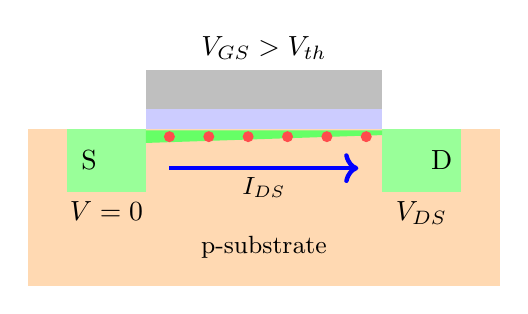
\begin{tikzpicture}[scale=1.0]
            % Substrate
            \fill[orange!30] (0,-2) rectangle (6,0);
            \node[font=\small] at (3,-1.5) {p-substrate};
            
            % Source/Drain 
            \fill[green!40] (0.5,-0.8) rectangle (1.5,0);
            \fill[green!40] (4.5,-0.8) rectangle (5.5,0);
            
            % Oxide 
            \fill[blue!20] (1.5,0) rectangle (4.5,0.25);
            
            % Gate 
            \fill[gray!50] (1.5,0.25) rectangle (4.5,0.75);
            
            % Channel at substrate surface 
            \fill[green!60] (1.5,-0.02) -- (1.5,-0.18) -- (4.5,-0.08) -- (4.5,-0.02) -- cycle;
            
            % Electrons
            \foreach \x in {1.8, 2.3, 2.8, 3.3, 3.8, 4.3} {
                \fill[red!70] (\x,-0.1) circle (0.07cm);
            }
            
            % Current arrow
            \draw[->, ultra thick, blue] (1.8,-0.5) -- (4.2,-0.5);
            \node[below, font=\small] at (3,-0.5) {$I_{DS}$};
            
            % Labels
            \node[left] at (1,-0.4) {S};
            \node[right] at (5,-0.4) {D};
            \node[above] at (3,0.75) {$V_{GS} > V_{th}$};
            \node[below] at (1,-0.8) {$V=0$};
            \node[below] at (5,-0.8) {$V_{DS}$};
            
        \end{tikzpicture}
        \end{center}
        
    \end{columns}
    
\end{frame}

\begin{frame}{Saturation Region}
    
    \begin{columns}[t]
    \column{0.48\textwidth}
        \textbf{Conditions}:
        \begin{itemize}
            \item $V_{GS} > V_{th}$ (channel exists)
            \item $V_{DS} \geq V_{GS} - V_{th}$ (pinch-off)
        \end{itemize}
        
        \textbf{Characteristics}:
        \begin{itemize}
            \item Channel pinched off near drain
            \item Used in amplifiers (constant current source)
            \item Output resistance $r_o$ is high
        \end{itemize}
        
        \vspace{0.1cm}
        
        \textbf{Equation With channel-length modulation $\lambda$}:
        $$I_{DS} = \frac{1}{2} \mu_n C_{ox} \frac{W}{L} (V_{GS}-V_{th})^2(1+\lambda V_{DS})$$
        
    \column{0.48\textwidth}
        \begin{center}
        \textbf{Device Cross-Section}
        
        \vspace{0.2cm}
        
        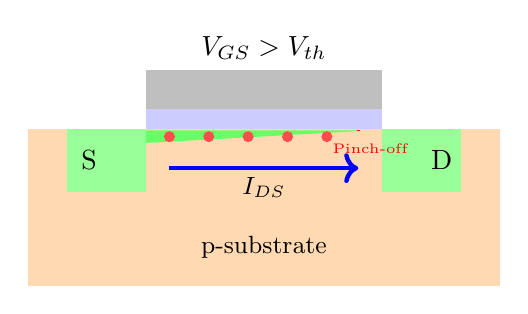
\begin{tikzpicture}[scale=1.0]
            % Substrate
            \fill[orange!30] (0,-2) rectangle (6,0);
            \node[font=\small] at (3,-1.5) {p-substrate};
            
            % Source/Drain 
            \fill[green!40] (0.5,-0.8) rectangle (1.5,0);
            \fill[green!40] (4.5,-0.8) rectangle (5.5,0);
            
            % Oxide 
            \fill[blue!20] (1.5,0) rectangle (4.5,0.25);
            
            % Gate 
            \fill[gray!50] (1.5,0.25) rectangle (4.5,0.75);
            
            % Channel at substrate surface 
            \fill[green!60] (1.5,-0.02) -- (1.5,-0.18) -- (4.2,-0.03) -- (4.2,-0.02) -- cycle;
            
            % Pinch-off region
            \draw[red, very thick] (4.2,-0.02) -- (4.2,-0.03);
            \node[font=\tiny, red] at (4.35,-0.25) {Pinch-off};
            
            % Electrons
            \foreach \x in {1.8, 2.3, 2.8, 3.3, 3.8} {
                \fill[red!70] (\x,-0.1) circle (0.07cm);
            }
            
            % Current arrow
            \draw[->, ultra thick, blue] (1.8,-0.5) -- (4.2,-0.5);
            \node[below, font=\small] at (3,-0.5) {$I_{DS}$};
            
            % Labels
            \node[left] at (1,-0.4) {S};
            \node[right] at (5,-0.4) {D};
            \node[above] at (3,0.75) {$V_{GS} > V_{th}$};
            
        \end{tikzpicture}
        \end{center}
        
    \end{columns}
    
\end{frame}

\section{I-V Characteristics}

\begin{frame}{Channel Length Modulation Effect}
    
    \begin{columns}[t]
    \column{0.48\textwidth}
        \textbf{Physical Mechanism}:
        
        \begin{itemize}
            \item In saturation, pinch-off point moves toward source
            \item Effective channel length decreases: $L_{eff} = L - \Delta L$
            \item $\Delta L$ increases with $V_{DS}$
            \item Current increases slightly with $V_{DS}$
            \item Finite output resistance
        \end{itemize}
        
        \textbf{Channel-Length Modulation Param.} ($\lambda$):
        
        \begin{itemize}
            \item Units: V$^{-1}$
            \item Typically 0.01 to 0.1 V$^{-1}$
            \item Smaller for longer channels
            \item Decreases with technology scaling
        \end{itemize}
        
    \column{0.48\textwidth}
        \textbf{Effect on I-V Characteristics}:
        
        \begin{center}
        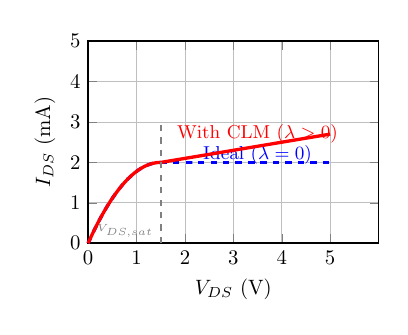
\begin{tikzpicture}[scale=0.75]
        \begin{axis}[
            width=6.5cm, height=5cm,
            xlabel={$V_{DS}$ (V)},
            ylabel={$I_{DS}$ (mA)},
            xmin=0, xmax=6,
            ymin=0, ymax=5,
            xtick={0, 1, 2, 3, 4, 5},
            ytick={0, 1, 2, 3, 4, 5},
            grid=major,
            thick,
            clip=false,
        ]
        
        % Linear region 
        \addplot[blue, ultra thick, dashed, domain=0:1.5, samples=50] {(8/3)*x - (8/9)*x^2};
        
        % Without CLM (ideal) - saturation
        \addplot[blue, ultra thick, dashed, domain=1.5:5, samples=50] {2};
        \node[font=\small, blue] at (axis cs:3.5,2.2) {Ideal ($\lambda=0$)};
        
        % With CLM - linear region
        \addplot[red, ultra thick, domain=0:1.5, samples=50] {(8/3)*x - (8/9)*x^2};
        
        % With CLM - saturation
        \addplot[red, ultra thick, domain=1.5:5, samples=50] {2*(1+0.1*(x-1.5))};
        \node[font=\small, red] at (axis cs:3.5,2.7) {With CLM ($\lambda>0$)};
        
        % Saturation boundary
        \draw[dashed, gray, thick] (axis cs:1.5,0) -- (axis cs:1.5,3);
        \node[font=\tiny, gray] at (axis cs:1.5,0.3) [anchor=east] {$V_{DS,sat}$};
        
        \end{axis}
        \end{tikzpicture}
        \end{center}
        
        \vspace{0.2cm}
        
        \textbf{Output Resistance}:
        $$r_o = \frac{\partial V_{DS}}{\partial I_{DS}} \approx \frac{1}{\lambda I_{DS}}$$
        
    \end{columns}
    
\end{frame}

\begin{frame}{$I_{DS}$ vs $V_{GS}$ Characteristics (Transfer Curve)}
    
    \begin{columns}[t]
    \column{0.48\textwidth}
        \textbf{Saturation Region} ($V_{DS}$ constant, large):
        
        $$I_{DS} = \frac{1}{2} \mu_n C_{ox} \frac{W}{L} (V_{GS}-V_{th})^2$$

        \begin{itemize}
            \item Quadratic relationship
            \item Threshold at $V_{GS} = V_{th}$
            \item Steeper for larger $W/L$
            \item Transconductance: $g_m = \frac{\partial I_{DS}}{\partial V_{GS}}$
        \end{itemize}
        
        \textbf{Transconductance}:
        $$g_m = \mu_n C_{ox} \frac{W}{L} (V_{GS}-V_{th})$$
        
        $$g_m = \sqrt{2 \mu_n C_{ox} \frac{W}{L} I_{DS}}$$
        
    \column{0.48\textwidth}
        \begin{center}
        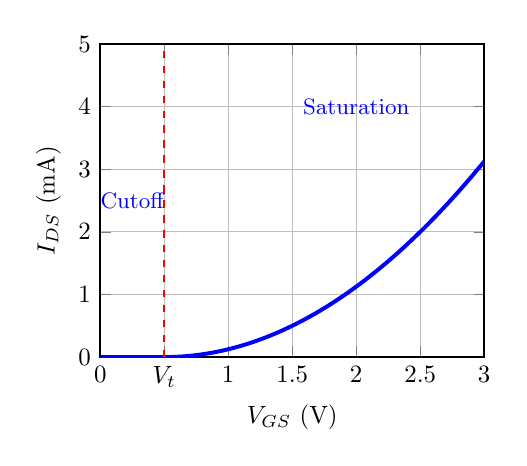
\begin{tikzpicture}[scale=0.9]
        \begin{axis}[
            width=7cm, height=6cm,
            xlabel={$V_{GS}$ (V)},
            ylabel={$I_{DS}$ (mA)},
            xmin=0, xmax=3,
            ymin=0, ymax=5,
            xtick={0, 0.5, 1, 1.5, 2, 2.5, 3},
            xticklabels={0, $V_t$, 1, 1.5, 2, 2.5, 3},
            ytick={0, 1, 2, 3, 4, 5},
            grid=major,
            thick,
        ]
        
        % Cutoff region
        \addplot[blue, ultra thick, domain=0:0.5, samples=20] {0};
        
        
        % Saturation region (quadratic)
        \addplot[blue, ultra thick, domain=0.5:3, samples=100] {0.5*(x-0.5)^2};
        
        % Threshold voltage line
        \draw[dashed, red, thick] (axis cs:0.5,0) -- (axis cs:0.5,5);
        \node[above, font=\small, red] at (axis cs:0.5,5) {$V_{th}$};
        
        % Regions
        \node[font=\small, blue] at (axis cs:0.25,2.5) {Cutoff};
        \node[font=\small, blue] at (axis cs:2,4) {Saturation};
        
        \end{axis}
        \end{tikzpicture}
        \end{center}
        
    \end{columns}
    
\end{frame}

\begin{frame}{$I_{DS}$ vs $V_{DS}$ Characteristics (Channel Length Modulation)}
    
    \begin{columns}[t]
    \column{0.35\textwidth}
        
        \textbf{Observations}:
        
        \begin{itemize}
            \item Each curve: constant $V_{GS}$
            \item Linear region: $I_{DS}$ increases with $V_{DS}$
            \item Saturation: $I_{DS}$ increases slightly due to CLM
            \item Higher $V_{GS}$ → higher $I_{DS}$
        \end{itemize}

        \textbf{Boundary} (dashed line):
        $$V_{DS} = V_{GS} - V_{th}$$
        
        \begin{itemize}
            \item Left: Linear/Triode region
            \item Right: Saturation region
        \end{itemize}

    
    \column{0.6\textwidth}


        \textbf{Saturation Region with CLM}
        $$I_{DS} = \frac{1}{2} \mu_n C_{ox} \frac{W}{L} (V_{GS}-V_{th})^2(1+\lambda V_{DS})$$
        \begin{center}
        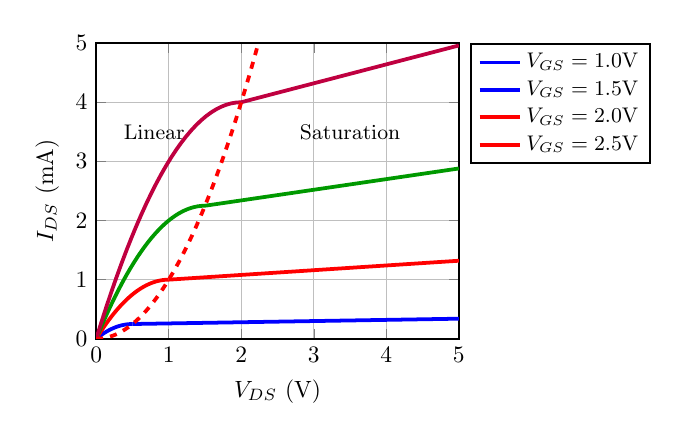
\begin{tikzpicture}[scale=0.85]
        \begin{axis}[
            width=7cm, height=6cm,
            xlabel={$V_{DS}$ (V)},
            ylabel={$I_{DS}$ (mA)},
            xmin=0, xmax=5,
            ymin=0, ymax=5,
            xtick={0, 1, 2, 3, 4, 5},
            ytick={0, 1, 2, 3, 4, 5},
            grid=major,
            thick,
            legend pos=outer north east,
            legend style={font=\small},
        ]
        
        % VGS = 1.0V (V_OV = 0.5V)
        \addplot[blue, ultra thick, domain=0:0.5, samples=30] {x - x^2};
        \addplot[blue, ultra thick, domain=0.5:5, samples=30] {0.25*(1+0.08*(x-0.5))};
        \addlegendentry{$V_{GS}=1.0$V}
        
        % VGS = 1.5V (V_OV = 1.0V)
        \addplot[red, ultra thick, domain=0:1.0, samples=30] {2*x - x^2};
        \addplot[red, ultra thick, domain=1.0:5, samples=30] {1.0*(1+0.08*(x-1.0))};
        \addlegendentry{$V_{GS}=1.5$V}
        
        % VGS = 2.0V (V_OV = 1.5V)
        \addplot[green!60!black, ultra thick, domain=0:1.5, samples=30] {3*x - x^2};
        \addplot[green!60!black, ultra thick, domain=1.5:5, samples=30] {2.25*(1+0.08*(x-1.5))};
        \addlegendentry{$V_{GS}=2.0$V}
        
        % VGS = 2.5V (V_OV = 2.0V)
        \addplot[purple, ultra thick, domain=0:2.0, samples=30] {4*x - x^2};
        \addplot[purple, ultra thick, domain=2.0:5, samples=30] {4.0*(1+0.08*(x-2.0))};
        \addlegendentry{$V_{GS}=2.5$V}
        
        % Saturation boundary (parabola: I = V_DS^2 along V_DS = V_GS - V_th)
        \addplot[red, dashed, ultra thick, domain=0:2.236, samples=50] {x^2};
        
        % Region labels
        \node[font=\small] at (axis cs:0.8,3.5) {Linear};
        \node[font=\small] at (axis cs:3.5,3.5) {Saturation};
        
        \end{axis}
        \end{tikzpicture}
        \end{center}
 
    \end{columns}
    
\end{frame}

\section{Summary}

\begin{frame}{Summary: MOSFET Structure and Operation}
    
    \begin{columns}[t]
    \column{0.45\textwidth}
        \textbf{Device Structure}:
        \begin{itemize}
            \item Four-terminal device (G, D, S, B)
            \item Gate controls channel via field effect
            \item n-channel: electrons, p-channel: holes
            \item $V_{th}$ (threshold voltage)
        \end{itemize}
        
        \vspace{0.3cm}
        
        \textbf{Operating Regions}:
        \begin{enumerate}
            \item \textbf{Cutoff}: $V_{GS} < V_{th}$, $I_{DS} = 0$
            \item \textbf{Linear}: $V_{DS} < V_{GS}-V_{th}$, resistor-like
            \item \textbf{Saturation}: $V_{DS} \geq V_{GS}-V_{th}$, current source
        \end{enumerate}
        
    \column{0.55\textwidth}
        \textbf{I-V Characteristics}:
        
        \begin{itemize}
            \item \textbf{Linear region}:
            $$I_{DS} = \mu_n C_{ox} \frac{W}{L}\left[(V_{GS}-V_{th})V_{DS} - \frac{V_{DS}^2}{2}\right]$$
            
            \item \textbf{Saturation region}:
            $$I_{DS} = \frac{1}{2}\mu_n C_{ox} \frac{W}{L}(V_{GS}-V_{th})^2(1+\lambda V_{DS})$$
        \end{itemize}
        
        \vspace{0.3cm}
        
        \textbf{Channel Length Modulation}:
        \begin{itemize}
            \item Finite output resistance in saturation
            \item $r_o \approx \frac{1}{\lambda I_{DS}}$
        \end{itemize}
        
    \end{columns}
    
\end{frame}

\begin{frame}{Key Parameters and Definitions}
    
    \begin{columns}[T]
    \column{0.48\textwidth}
    \begin{table}[t]
    \centering
    \renewcommand{\arraystretch}{1.8}
    \small
    \begin{tabular}{|l|p{4cm}|}
    \hline
    \textbf{Parameter} & \textbf{Description} \\
    \hline
    \hline
    $V_{th}$ & Threshold voltage \\
    \hline
    $V_{GS}$ & Gate-source voltage \\
    \hline
    $V_{DS}$ & Drain-source voltage \\
    \hline
    $V_{OV}$ & Overdrive: $V_{GS}-V_{th}$ \\
    \hline
    $W/L$ & Aspect ratio \\
    \hline
    \end{tabular}
    \end{table}
    
    \column{0.48\textwidth}
    \begin{table}[t]
    \centering
    \renewcommand{\arraystretch}{1.8}
    \small
    \begin{tabular}{|l|p{4cm}|}
    \hline
    \textbf{Parameter} & \textbf{Description} \\
    \hline
    \hline
    $\mu_n$ & Electron mobility \\
    \hline
    $C_{ox}$ & Oxide capacitance per unit area \\
    \hline
    $\lambda$ & Channel-length modulation \\
    \hline
    $g_m$ & Transconductance \\
    \hline
    $r_o$ & Output resistance \\
    \hline
    \end{tabular}
    \end{table}
    \end{columns}
    
\end{frame}

\end{document}
